\chap{States: Don't Always Do the Same Thing (Advanced)}\label{ch.states}

A program in VPL is a list of event-action pairs. All the events are
checked periodically and the appropriate actions are taken.
This limits the programs that we can create; to go further we
need a way to specify that certain
event-action pairs are active at a certain time, while others are not.
For example, in \cref{ch.line}, when the robot ran off the tape,
we wanted it to turn left or right in order to search for the tape with
the direction depending on which side it ran off.

States are supported in the \emph{advanced} mode of VPL. Click on
\blksm{advanced} before beginning to work on the following projects.

\sect{Tap, tap}

In many programs, we used one button to start the robot's behavior and
another to stop it. Consider, though, the power switch on my computer:
%\blksm{power-button}:
The same switch is used to turn the light on and
off; the switch \emph{remembers} whether it is in the state \bu{on} or the
state \bu{off}. The switch often includes a small green light which indicates
its current state.

Write a program that turns the robot's lights on when it is tapped and
turns them off when tapped again.

{\raggedleft \hfill Program file \bu{tap-on-off.aesl}}

It is convenient to display the required behavior in a \textit{state diagram}:

\begin{center}
\begin{picture}(240,45)
\thicklines
%\put(0,0){\framebox(240,40){}}
\put(20,20){\circle{40}}
\put(0,0){\makebox(40,40){\textsf{off}}}
\put(220,20){\circle{40}}
\put(200,0){\makebox(40,40){\textsf{on}}}
\put(40,30){\vector(1,0){160}}
\put(0,30){\makebox(240,10){\textsf{tap $\rightarrow$ turn on}}}
\put(200,10){\vector(-1,0){160}}
\put(0,10){\makebox(240,10){\textsf{tap $\rightarrow$ turn off}}}
\end{picture}
\end{center}

In the diagram there are two states indicated by circles labeled with
the names of the states \bu{off} and \bu{on}. From state \bu{off} the
robot can go to state \bu{on} and back, but only by following the
instructions on the arrows. The instructions describe when a transition
from one state to another can occur and what happens when it does occur:

\begin{itemize}

\item \emph{When} the robot is in state \bu{off} \textbf{\textit{and}}
the \emph{tap} event occurs $\rightarrow$ turn the lights \emph{on}
\textbf{\textit{and}} go to state \bu{on}.

\item \emph{When} the robot is in state \bu{on} \textbf{\textit{and}}                                                                                                                        
the \emph{tap} event occurs $\rightarrow$ turn the lights \emph{off}                                                                                                                         
\textbf{\textit{and}} go to state \bu{off}. 

\end{itemize}

The emphasized word ``\textbf{\textit{and}}'' before the arrow~$\rightarrow$
means there are two conditions that must be true in order for the
transition to be taken. (a) The robot must be in a certain state and (b)
the event must occur. When both conditions are true, the transition is taken,
causing both the state to change and the action written after the arrow~$\rightarrow$ to be performed.

It is important to realize that the two parts of the condition are
independent. In the above diagram (repeated here):

\begin{center}
\begin{picture}(240,45)
\thicklines
%\put(0,0){\framebox(240,40){}}
\put(20,20){\circle{40}}
\put(0,0){\makebox(40,40){\textsf{off}}}
\put(220,20){\circle{40}}
\put(200,0){\makebox(40,40){\textsf{on}}}
\put(40,30){\vector(1,0){160}}
\put(0,30){\makebox(240,10){\textsf{tap $\rightarrow$ turn on}}}
\put(200,10){\vector(-1,0){160}}
\put(0,10){\makebox(240,10){\textsf{tap $\rightarrow$ turn off}}}
\end{picture}
\end{center}

the event \emph{tap} appears twice, but the action caused by the
occurrence of this event \emph{depends on} which state the robot is in.

Similarly, in a single state, different events can cause different
actions and transitions to different new states. In the following
diagram:

\begin{center}
\begin{picture}(240,80)
\thicklines
%\put(0,0){\framebox(240,80){}}
\put(30,42){\circle{30}}
\put(14,28){\makebox(30,30){\textsf{off}}}
\put(220,22){\circle{30}}
\put(205,8){\makebox(30,30){\textsf{on2}}}
\put(40,57){\vector(1,0){160}}
\put(220,60){\circle{30}}
\put(205,45){\makebox(30,30){\textsf{on1}}}
\put(40,27){\vector(1,0){160}}
\put(0,60){\makebox(240,10){\textsf{left button $\rightarrow$ turn green}}}
\put(0,30){\makebox(240,10){\textsf{right button $\rightarrow$ turn red}}}
\end{picture}
\end{center}

touching the left button in the state \textbf{off} causes the green
light to be turned on and a change to state \textbf{on1}, whereas
touching the right button \emph{in the same state} causes a different
action, the red light is turned on, and a change to a different state, \textbf{on2}.

\sect{Implementing state diagrams with event-action pairs}

We show how to implement the behavior described by a state diagram as event-action pairs.
To implement means to create a program that will do what the state diagram describes.
The program is shown in \cref{fig.turn-on-off}. Let us look
at the event-action pairs one-by-one.

\begin{figure}
	\subfigure[Tap to turn on and off]{
		\label{fig.turn-on-off1}
		\includegraphics[width=.4\textwidth]{tap-on-off1}
	}
	\hfill
	\subfigure[Tap to change the state]{
		\label{fig.turn-on-off2}
		\includegraphics[width=.4\textwidth]{tap-on-off2}
	}
	\caption{Tap has a different result depending on a state}
	\label{fig.turn-on-off}
\end{figure}

In the first event-action pair, the event is composed of the
tap block together with an indication of the state \blksm{tap-turn-on-state-only}: \blkc{tap-turn-on}

A state is indicated by four quarters of a circle, each of which can be
either on (orange) or off (white). In this program, we will use the left-front quarter to
indicate whether the robot's top light is off or on. In this pair, this
quarter is colored white, meaning that the robot's light is off.
Therefore, the meaning of the this pair is: if the robot is tapped and the light is off, turn
it on.

Similarly, the second event-action pair means: if the robot
is tapped and the light is on, turn it off: \blkc{tap-turn-off}
% . The quarter is colored orange, meaning that the robot's light is on

If you look again at the state diagram, you
will see that only half the job is done. Indeed, when turning the light on or
off, we also have to change the state of the robot from \bu{off} to
\bu{on} or from \bu{on} to \bu{off}. For that we create two
additional event-action pairs using the \emph{state} action block
\blksm{action-states}, as shown in \cref{fig.turn-on-off2}.

The meaning of the first one is: \emph{when} the robot is tapped
\emph{and} the state is \bu{off}, change the state to \bu{on}:
\blkc{tap-state-on}
Similarly, the meaning of the second one is \emph{when} the robot
is tapped \emph{and} the state is \bu{on}, change the state to \bu{off}: \blkc{tap-state-off}

Referring the complete program consisting of the four pairs in \cref{fig.turn-on-off}, we see that
each event causes both an action on the light and a change of the state
of the robot. Both the action and the change of state depend on the state the robot is in, called \emph{current state}.

\newpage

\sect{How many states can the robot be in?}

The state is indicated by a circle divided into four quarters.
When used with an event or in the state action block, each quarter can be:
\begin{itemize}
\item \textbf{White}: the quarter is \emph{off};
\item \textbf{Orange}: the quarter is \emph{on};
\item \textbf{Gray}: the quarter is ignored.
\end{itemize}

For example, in \blksm{states}, the left-front and right-rear quarters are on, the
right-front one is off and the left-rear one is not taken into account,
meaning that if \blksmpure{states} is associated with an event block, the
event will occur if the state is either set to:
\begin{center}
\centering \makebox{\raisebox{-1.7em}{\includegraphics[height=4em]{states1}}}\quad or \quad \makebox{\raisebox{-1.7em}{\includegraphics[height=4em]{states2}}}
\end{center}

Since each of the four quarters can be either on or off, there are 2 $\times$ 2 $\times$ 2 $\times$ 2 = 16 possible states:
\begin{quote}
\bu{(off, off, off, off)\\(off, off, off, on)\\(off, off, on, off)\\
\mbox{}\hspace{3em}\ldots\\
(on, on, on, off)\\
(on, on, on, on)}.
\end{quote}
\Cref{fig.all-states} enumerates graphically all these states.
The current state of the robot is always displayed on the top of the robot by bright circle arcs, for instance, \cref{fig.state-leds} shows the robot in the state \bu{(on, on, on, on)}.

\trickbox[Information]{When a program is run, the initial state is
\bu{(off, off, off, off)}:\quad \blk{state-all-off}}

\trickbox{If you do not use all possible 16 states, but for instance only 2 or 4, you are free to decide which quarters you use to represent your state.
Also, if for instance you have two different things you want to encode in the state, and each of them have two possible values, you can use two quarters independenly.
That is why the ability to \emph{ignore} a quarter is very useful!
Try to always stay as simple as possible.
}

\begin{figure}
	\subfigure[All possible states of Thymio]{
		\label{fig.all-states}
		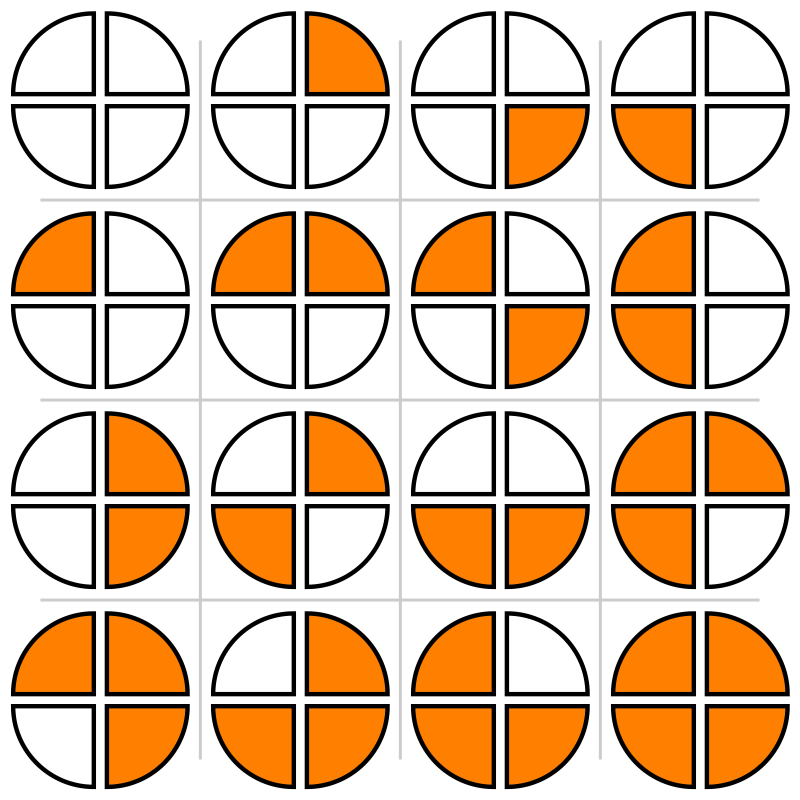
\includegraphics[width=.4\textwidth]{all-states}
	}
	\hfill
	\subfigure[The LED circle indicates the state]{
		\label{fig.state-leds}
		\includegraphics[width=.4\textwidth]{state-leds}
	}
	\caption{The states of Thymio and their representation}
\end{figure}

\sect{Get the mouse}

Write a program that causes the robot to turn from right to left,
searching for a mouse (or another object).
If the robot detects a mouse with its leftmost sensor it
continues the search until the mouse is detected by its rightmost
sensor. Then, it positions itself facing the mouse, as shown in \cref{fig.cat-mouse}.

{\raggedleft \hfill Program file \bu{mouse.aesl}}

\begin{figure}
	\subfigure[The cat has found the mouse]{\label{fig.cat-mouse}
	\includegraphics[width=0.4\textwidth]{cat-mouse}}
	\hfill
	\subfigure[Searching with the rightmost sensor]{\label{fig.mouse2}
	\includegraphics[width=0.4\textwidth]{mouse2}}
	\caption{The robot cat is looking for the mouse}
\end{figure}

The following event-action pair causes the robot to turn left: \blkc{mouse1}
This only occurs when the left-front quarter is off; initially all
quarters of the state are off.

The first event-action pair in \cref{fig.mouse2} waits until the
mouse is detected at the rightmost sensor. Note that the small square
next to it is colored white so that the event occurs only when the
rightmost sensor alone detects the mouse. The second event-action pair
in the \cref{fig.mouse2} changes the state.

The final event-action pair in the program halts the robot when the mouse is directly facing the center
sensor: \blkc{mouse3}
Why does the event in this pair need to depend on the state? The reason
is that the central sensor will also detect the mouse in its initial
scan from right to left. We want the robot to perform a full scan
before returning to the position of the mouse, so it is necessary that
this first detection of the mouse be ignored. This is achieved by
stopping the scan only when the state is \bu{on} and this is set only
when the full scan has been completed.

\vfill

\trickbox{
You will have to experiment with the distance of the mouse to the robot.
If it is too close to the robot, the sensors on either side of
the central sensor will also detect the mouse, while the event requires
that they \emph{not} detect it.}

\vfill

\exercisebox{\thechapter.1}{
Write a program that causes the robot to dance: it turns left in
place for two seconds and then turns right in place for three seconds.
These movements are repeated indefinitely.
}

\exercisebox{\thechapter.2 (Difficult)}{
Modify the line-following program from \cref{ch.line} so that the
robot turns left when it leaves the right-hand side of the line and
turns right when it leaves the left-hand side of the line.
}